\documentclass[conference]{IEEEtran}
% \IEEEoverridecommandlockouts
% The preceding line is only needed to identify funding in the first footnote. If that is unneeded, please comment it out.


\usepackage{soul}
\usepackage{amsmath, amssymb, amsfonts}
\usepackage{algorithmic}
\usepackage{graphicx}
\usepackage{textcomp}
\usepackage{xcolor}

\usepackage{caption}
\usepackage{subcaption}
\usepackage{cleveref}

% \usepackage{cite}
\usepackage{amsmath,amssymb,amsfonts}
\usepackage{algorithmic}
\usepackage{graphicx}
\usepackage{textcomp}
\def\BibTeX{{\rm B\kern-.05em{\sc i\kern-.025em b}\kern-.08em
    T\kern-.1667em\lower.7ex\hbox{E}\kern-.125emX}}

\usepackage[backend=biber,style=ieee]{biblatex}
\addbibresource{references.bib}

% Define new environments
\usepackage{amsthm}
\newtheorem{theorem}{Theorem}
\theoremstyle{definition}
\newtheorem{definition}{Definition}

\begin{document}


\title{Nonlinear Model Reference Adaptive Control (NMRAC) for Multiple-Input, Multiple-Output Systems}
% max 15 words



\author{\IEEEauthorblockN{Dalim Wahby}
\IEEEauthorblockA{ \textit{Université Côte d'Azur}\\
\textit{I3S/CNRS}\\
Sophia Antipolis, France \\
wahby@i3s.unice.fr}
\and
\IEEEauthorblockN{Alvaro Detailleur}
\IEEEauthorblockA{\textit{IDSC} \\
\textit{ETH Zürich}\\
Zürich, Switzerland \\
adetailleur@student.ethz.ch}
\and
\IEEEauthorblockN{Christopher Onder}
\IEEEauthorblockA{\textit{IDSC} \\
\textit{ETH Zürich}\\
Zürich, Switzerland \\
onder@idsc.mavt.ethz.ch}
\and
\IEEEauthorblockN{Guillaume Ducard}
\IEEEauthorblockA{ \textit{Université Côte d'Azur}\\
\textit{I3S/CNRS}\\
Sophia Antipolis, France \\
ducard@i3s.unice.fr}
}
\maketitle

\begin{abstract}
    \hl{...}
    \newline
\end{abstract}

\begin{IEEEkeywords}
    Neural Networks, Gradient Descent, Control, Lyapunov Method 
\end{IEEEkeywords}
\section{Introduction}
Model reference control is a technique that imposes a behavior on a system, by equating the the output of the model reference with the output of the controlled system. This way, the gains of a pre-defined controller structure can be found. 

However, this only works if the system's dynamics are known exactly, which is often far from reality. If the system's dynamics are not fully known, the controller gains can be found adaptively by a technique called \textit{model reference adaptive control} (MRAC). The adaptation law can be chosen in two ways, firstly a gradient descent-based update law as first proposed by Whitaker et al. \cite{whitaker1959adaptive} and applied in for example \textbf{wahby} \cite{bosshartComparisonTwoPID2021}, and secondly, a Lyapunov-based update law as proposed by Shackcloth et al. \cite{shackclothSynthesisModelReference1965}. The latter enforces that in every update step, we have a stabilizing controller, which is not guaranteed when using the former.

Since the structure of the control law is pre-defined, a rich enough model has found. To this end, neural networks (NN) are an ideal choice, since they are considered to be universal approximators \cite{hornikUniversalApproximationUnknown1990a}. Since at least the 90s, research has been conducted on NN controllers \cite{jiangBriefReviewNeural2017}, and it has been shown that they can learn a desired behavior, for example in \textbf{wahby} \cite{congPIDLikeNeuralNetwork2009,thanhNonlinearPIDControl2006,norrisNeuralNetworksControl2021}. However, standard NNCs are nonlinear, through the use of nonlinear activation functions, which makes their makes the formal verification of stability more challenging. Often these controllers rely on a posteriori stability verification, \hl{...}

which can become non-trivial or is not enough if we require online, stable learning techniques.

To ensure that a system engages in the desired behavior, we need to assess its stability, meaning we need to mathematically analyze and verify if a system converges to the desired output, given the input signal. If this is the case, we say the system is stable. While classical control theory primarily deals with linear time-invariant (LTI) systems, following the superposition principle, real-world systems often exhibit nonlinear behavior. This extends the scope of traditional control theory to handle these more complex, nonlinear systems, which leads us to not be able to use classical stability concepts, such as gain and phase margins. Hence, we need to use more generalized methods, such as Lyapunov theory, which aims to quantify dissipative energy in the system. However, finding an appropriate Lyapunov function can be challenging. When using MRACs with a Lyapunov-based update law, we can impose a Lyapunov function and ensure that the weights satisfy stability conditions on this function. In the MRAC literature however, this is only done for adaptive weights that appear in the form of a linear combination with the error dynamics of the system, meaning the learned parameters are not inside the nonlinear function. Hence, in this work we aim to extend on the MRAC principle and define a nonlinear update rule for MRAC controllers, where the estimated parameters are in a function that does not satisfy the superposition principle.

To this end, we first investigate the performance of stable linear MRACs compared to existing, not necessarily stable learning schematics, such as a PIDNN and a self-tuning PID controller, applied to an inverted pendulum, called Pendubot. With our insights on developing stable linear MRACs, we go ahead and tackle the problem of stable nonlinear MRACs. For reasons of simplicity, we begin by defining an update law for a first-order system and subsequently propose a MIMO update law. Both newly proposed update laws will are validated through simulations.
\subsection{Literature Review}
\label{sec:related-work}
Model Reference Adaptive Control (MRAC) was first introduced in the early 1970s by Whitaker et al. \cite{whitakerDesignModelReference1958}. Originally, it was thought to deal with process uncertainties and disturbance dynamics, however, the proposed techniques were also used in different contexts, including but not limited to auto-tuning, automatic construction of gain schedules, and adaptive filtering \cite{astromTheoryApplicationsAdaptive1983, astromHistoryAdaptiveControl2014}.

The adaptation mechanism of the controller parameters follows two main approaches, namely 1) the MIT method or gradient descent-based method, and 2) the Lyapunov method \cite{astromAdaptiveControl2008}. The MIT method does not come with stability guarantees \cite{mareelsRevisitingMitRule1987}, whereas the Lyapunov method is based on an adaptation rule derived from Lyapunov's second method \cite{shackclothSynthesisModelReference1965}. It imposes stability since the adaptation rule is chosen in a way such that the decrease condition on the Lyapunov function is always satisfied, thus, implying system convergence.

Generally, MRACs can be split into three categories, firstly direct and secondly indirect MRAC. The former aims to adapt controller parameters directly and the latter aims to update the model parameters. The third category is a hybrid approach called \textit{Combined/Composite MRAC}, first proposed by Duarte et al. in \cite{duarteCombinedDirectIndirect1989} for first-order systems. The approach is based on estimating two parts with two separate adaptation rules, namely 1) unmatched model uncertainty and 2) system parameters. Their approach showed in simulations to be more robust than both direct and indirect adaptive control if considered individually \cite{narendraRobustAdaptiveControl1988}, however, this has yet to be proven. Combined MRACs are generalizable for $n$-th order linear systems, as proposed by Lavretsky and Tao et al. \cite{taoAdaptiveControlSystems2013}. Additionally, Lavretsky proposes Combined MRACs using RBF NNs to perform system identification and estimate the unmatched uncertainties model, with proven stability guarantees, which enables us to apply this method to a larger class of nonlinear systems \cite{lavretskyCombinedCompositeModel2009}.

The porposed algorithm is a direct MRAC method, utilizing a Lyapunov-based learning mechanism, that includes nonlinearities in the form of a simple feedforward NN.

% Simultaneously, Slotine et al. developed a similar approach, called \textit{Composite MRAC} \cite{slotineAdaptiveControlRobot1987a, slotineAdaptiveRobotControl1987, slotineAppliedNonlinearControl1991}, extending MRACs to a class of nonlinear systems, where the estimated parameters appear linearly in the known, nonlinear dynamics of the system. Applications of the approaches proposed by Narendra et al. and Slotine et al. have shown to be effective and include but are not limited to \cite{duarte-mermoudExperimentalEvaluationCombined2002,duarte-mermoudControlLongitudinalMovement2005}.

% In 2000, Patiño et al. proposed to leverage indirect MRACs to adaptively compensate for nonlinearities in the plant \cite{patinoNeuralNetworkbasedModel2000}. They propose to use Radial Basis Functions (RBF), whose parameters are adapted, to compensate for nonlinearities in the system. This approach can be considered as adaptive nonlinear dynamic inversion (ANDI). A similar ANDI approach was published in \cite{karnalasadanNeuralNetworkBased2004}.

% Furthermore, Lavretsky uses a Linear Quadratic Regulator (LQR) regulator as a reference model, ensuring optimality of the control law. However, due to the design of an LQR, the states and control input of the system cannot be constrained, meaning if the system has physical constraints they are not accounted for in the control strategy. Similar approaches were proposed in \cite{joshiDeepModelReference2019, trisantoApplicationNeuralNetworks2006, slamaModelReferenceAdaptive2018}.


\subsection{Contributions}
\label{sec:contributions}
The method proposed in this work is based on the logic of the perviously mentioned works and the novelty of this apporach lies in the ability of learning a stabilizing controller, despite of a nonlinear NN being present in the closed-loop system. Additionally, the propsed algorithm is validated in simulation, which show the convergence of the NN parameters to their desired values.
\section{Definitions and nomenclature}
\label{sec:definitions}
\subsection{Systems and Stability}
In order to define stable learning algorithms, it is imperal to firstly define, first-order systems and stability, which is taken from \cite{khalilNonlinearSystems1996}.

\begin{definition}[First-Order System]
    A continuous-time first-order system is defined by the following map
    \begin{equation}
        f:\mathbb{R}\times\mathbb{R}\rightarrow \mathbb{R}, (x(t),u(t)) \mapsto \dot x(t) = f(x(t),u(t)).
        \label{def:eq-system}
    \end{equation}

    Additionally, if $u(t)$ is a function of $x$, the system is autonomous, with closed-loop dynamics $f(x(t)$). The trajectory of the system is defined by the evolution of $x(t)$ over time. Furthermore, the system has an equilibrium point at $f(x(t))=0$.
    \label{def:system}
\end{definition}

\begin{definition}[Stability]
    Consider the equilibrium point $x=0$ of \eqref{def:eq-system}. Then the system is... 
    \begin{itemize}
        \item \textit{stable}, if for each $\epsilon>0$, there is a $\delta>0$, such that
            $$||x(0)||<\delta \Rightarrow ||x(t)||<\epsilon, \quad \forall t \geq 0$$ 
        \item \textit{unstable}, if not stable, and
        \item \textit{asymptotically stable} if it is stable and $\delta$ can be chosen such that
            $$||x(0)||<\delta \Rightarrow \lim_{t\rightarrow\infty} x(t)=0 $$
    \end{itemize} 
\end{definition}
From here henceworth, the dependency of the dynamics on time is considered to be implicit and will be neglected in the notation.


\begin{definition}[Lyapunov function]
    A Lyapunov function is a continuous function $V: \mathbb{R}^n\rightarrow\mathbb{R}$ with the following properties:
    \begin{enumerate}
        \item[(a)] positive definitness: $V(x)>0, \quad \forall x\in\mathbb{R}^n\setminus\{0\}$ and $V(0)=0$,
        \item[(b)] decrease condition: $\dot V(x)\leq0, \quad \forall x\in\mathbb{R}$.
    \end{enumerate}
\end{definition}

\begin{definition}[Stability in the sense of Lyapunov]
    If there exists a continuous function $V: \mathbb{R}^n \rightarrow \mathbb{R}$ such that
     \begin{enumerate}
       \item[(a)] $V(x)$ is positive definite, and
       \item[(b)] $\dot{V}(x)\leq-l(x)$, for some positive semidefinite function $l(x)$,
     \end{enumerate}
    then the system is considered to be stable. Additionally, if $l(x)$ is positive definite, then the system is asymptotically stable.
     \label{def:lyapunov-stability}
\end{definition}

The ultimate goal of this work is to develop stable update laws for NNCs. Hence, the designed control law will be considered as a NN. Therefore, throughout this work NNs are defined as follows.

\begin{definition}[Neural network]
    A neural network (NN) $\phi:\mathbb{R}^n\rightarrow \mathbb{R}^p$ is defined as:
   
     \begin{equation}
      \begin{aligned}
        \phi (x) & = (L_1 \circ \varphi_1 \dots \circ L_{H-1} \circ \varphi_{H-1} \circ L_{H} \circ \varphi_H)(x)\\
        L_i(x) &= \theta_i x + b_i \quad \forall i\in\{1,..., H\},
      \end{aligned}
    \end{equation}
     where $\varphi_i(\cdot)$ are called  activation functions, $\theta_i$ and $b_i$ are the weight matrix and bias of layer $i$, respectively. Whenever, a bias is not mentioned it is assumed to be zero.
\end{definition}

NNs usually make use of nonlinear activation functions, which enable them to approximate nonlinear functions. Typically, functions such as the hyperbolic tangent, sigmoid, or ReLU are used in machine learning. This work will utilize an actiavtion function that is designed to model a smooth saturation function, as used in \cite{wahby, thanhNonlinearPIDControl2006} and defined in \eqref{eq:sigmoid}. Note, that it activation function saturates at $\pm \frac{2}{a}$.

\begin{equation}
    \sigma (x) = \frac{2(1-e^{-ax})}{a(1+e^{-ax})}
    \label{eq:sigmoid}
\end{equation}


\section{Nonlinear Model Reference Adaptive Control (NMRAC)}
\label{sec:NMRAC}

Direct MRAC is charaterized by the controller parameters being direclty updated through an update mechanism, which takes into acount the error of the system with respect to the desired output, as shown in Fig. \ref{fig:nonlinear-NNC-MRAC}. The porposed approach is a Lyapunov-based approach that defines the update mechanism based on a Lyapunov candidate. In this Section, the NMRAC problem for first-order systems is defined.

\begin{figure}[!t]
    \centering
    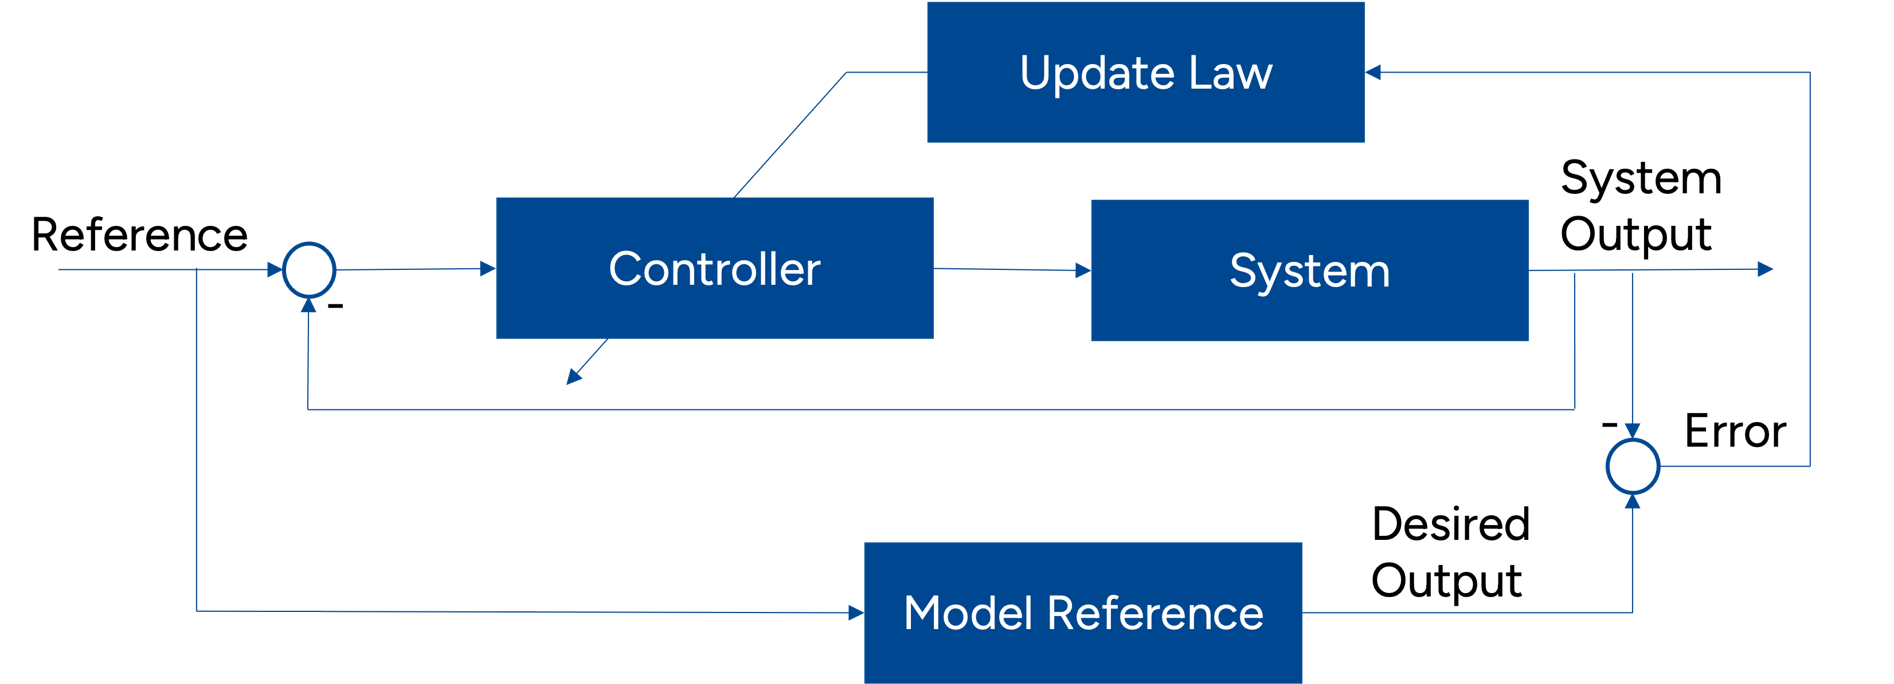
\includegraphics[width=0.8\linewidth]{images/MRAC_Blockdiagram.png}
    \caption{MRAC for first-oder systems controlled by simple NNCs}
    \label{fig:nonlinear-NNC-MRAC}
\end{figure}

% In this work a stable update scheme is proposed for first-order systems. More, specifically, a problem is defined, where we show that the even in the nonlinear case, we are able to learn a parameter with an algorithm that is based on the logic of a linear MRAC. We call this nonlinear Model Reference Adaptive Control (NMRAC).

The system to control is of the form, as described in equation \eqref{eq:first-order-system}, where $\phi: \mathbb{R}\rightarrow\mathbb{R}$ is a nonlinear function, $e_x=x_r - x$, and $\theta$ is an adaptable parameter. It can be seen as a weight of  NN, with actiavtion function $\phi$, as defined in \eqref{eq:sigmoid}. 

\begin{equation}
    \dot x = -ax + b\phi(\theta e_x)
    \label{eq:first-order-system}
\end{equation}

Next, a stable model reference is defined, as per equation \eqref{eq:first-order-ref}, where $e_m=x_r - x_m$, and $a_m>0$.

\begin{equation}
    \dot x_m = -a_mx_m + b_m\phi_m(\theta_m e_m)
    \label{eq:first-order-ref}
\end{equation}

Since the goal is, that the system learns the behavior of the model reference, error dynamics are defined as follows. 
\begin{equation}
    e=x_m-x
    \label{eq:error-dynamics-nonlinear}
\end{equation}
Note, that from this definition it follows that $e=e_x-e_m$, which is used as an alternative definition for the stability analysis of the update law later on in this work.

Following the error dynamics, a Lyapunov candidate is defined, as in equation \eqref{eq:nonlinear-lyapunov-candidate}.
\begin{equation}
    V(e, \alpha) =||e||_2^2 + ||c \alpha||_2^2
    \label{eq:nonlinear-lyapunov-candidate}
\end{equation}
The factor $c>0$ can be considered to be the learning rate, which is used to accelerate or decelerate the learning process. The norm of the error captures the distance between the internal states of the reference model and the system, and the term $||\alpha||_2^2$ captures the distance between the NNC and the desired NNC, which can be seen as the difference in dynamics between the controlled system and the model reference. Note, that both $e$ and $\alpha$ should be $0$, when the system follows the model reference and the desired parameters are learned. Futhermore, this property renders our Lyapunov candidate to be positive definite.

To ensure that the controlled system is stable, a negative time derivative of the Lyapunov function is required. Therefore, we analyze the behavior of the resulting time derivative of the Lyapunov function. The resulting equation is defined by:
\begin{equation}
    \begin{aligned}
    \dot V(e, \alpha) = & 2e\dot e + 2\alpha \dot \alpha c
    \end{aligned}
    \label{eq:nonlinear-lyapunov-derivative}
\end{equation}

The time derivative of the error dynamics are defined by \eqref{eq:nonlinear-error-time-derivative}. The equation is extended by $\pm (a_mx b_m \phi_m(\theta_m e_x))$, to construct the term $\alpha$, which is now dependent on $e_x$, and $\theta$. Two term remain, namely, $-a_me$, and $\gamma_m(e_m, e_x)$.

\begin{equation}
    \begin{aligned}
    \dot e 
= & \dot x_m - \dot x \\ 
= & -a_mx_m + b_m\phi_m(\theta_me_m) - (-ax + b\phi(\theta e_x)) \\
    & \pm (a_mx + b_m \phi_m(\theta_m e_x)) \\
    = & -a_m \underbrace{(x_m-x)}_{=e} \\ 
    & + \underbrace{(a-a_m)x+b_m\phi_m(\theta_me_x) - b\phi(\theta e_x)}_{=\alpha(e_x, \theta)} \\ 
    & + \underbrace{b_m(\phi_m(\theta_m e_m)-\phi_m(\theta_m e_x))}_{=\gamma_m(e_m,e_x)}
    \end{aligned}
    \label{eq:nonlinear-error-time-derivative}
\end{equation}

Through substitution of \eqref{eq:nonlinear-error-time-derivative} into \eqref{eq:nonlinear-lyapunov-derivative}, equation \eqref{eq:nonlinear-lyapunov-derivative2} is obtained.
\begin{equation}
    \begin{aligned}
    \dot V(e, \alpha) 
    = & 2e(-a_me + \alpha(e_x, \theta) + \gamma_m(e_m, e_x)) + 2\alpha c \dot \alpha(e_x, \theta)\\
    = & -2a_me^2 \\ 
    & + 2e\gamma_m(e_m, e_x) 
    \\ 
    & + 2\alpha(e_x, \theta)(e + c \dot \alpha(e_x, \theta))
    \end{aligned}
    \label{eq:nonlinear-lyapunov-derivative2}
\end{equation}
Note, that the first term $-2a_me^2$ is always negative, since $a_m>0$, and $e^2 > 0$. The second term will always be negative, due to the property of $e=e_x-e_m$. It follows that if $e<0 \Rightarrow \gamma_m(e_m, e_x)>0$, which implies that the second term is negative, and if $e>0 \Rightarrow \gamma_m(e_m, e_x)<0$, which again implies that the second term is negative. Hence, the second term always stays negative.

It remains to show that the last term does not influence equation \eqref{eq:nonlinear-lyapunov-derivative2} such that it changes sign. Since $\theta$ is dependent on time, this implies $\dot \alpha(e_x, \theta)$ will include a $\dot \theta$ term. Therefore, $\dot \theta$ is chosen, such that the third term is nullified. Note, that due to the way the update law is constructed, stability is guaranteed, since the Lyapunov function is positive definite and simultaneously the decrease condition is satisfied. The resulting update law is constructed as follows.

% \begin{equation}
%     \begin{aligned}
%         0 = & 2\alpha(e_x, \theta)(e +  \dot \alpha(e_x, \theta)) \\
%         \Leftrightarrow 0 = & e +  c \dot \alpha(e_x, \theta) \\
%         \Leftrightarrow 0 = & e + c \left[ (a-a_m)\dot x +b_m \frac{d\phi_m(\theta_me_x)}{dt} - b \frac{d\phi(\theta e_x)}{d t} \right]\\
%         \Leftrightarrow 0 = & \frac{1}{c}e + (a-a_m)\dot x +b_m \frac{\partial \phi_m(\tilde x)}{\partial \tilde x}\vert_{\tilde \theta e_x = \theta e_x}\theta_m \dot e_x - b \frac{d\phi(\tilde x)}{\partial \tilde x}\vert_{\tilde x = \theta e_x}(e_x \dot\theta + \theta \dot e_x)
%     \end{aligned}
% \end{equation}

% \begin{equation}
%     \begin{aligned}
%         0 = & 2\alpha(e_x, \theta)(e +  \dot \alpha(e_x, \theta))
%     \end{aligned}
% \end{equation}

% \begin{equation}
%     \begin{aligned}
%      \dot \theta = & \frac{1}{e_x b \frac{\partial \phi(\tilde x)}{\partial \tilde x}\vert_{\tilde x=\theta e_x}}\\ 
%      & (  \frac{1}{c} e + (a-a_m)\dot x + b_m\frac{\partial \phi_m(\tilde x)}{\partial \tilde x}\vert_{\tilde x=\theta_me_x}\theta_m \dot e_x) \\ 
%     & - \frac{\theta}{e_x}\dot e_x
%     \end{aligned}
%     \label{eq:nonlinear-update-law}
% \end{equation}

\begin{equation}
     \dot \theta = \frac{(\frac{1}{c} e + (a-a_m)\dot x + b_m\frac{\partial \phi_m(\tilde x)}{\partial \tilde x}\vert_{\tilde x=\theta_me_x}\theta_m \dot e_x) }{e_x b \frac{\partial \phi(\tilde x)}{\partial \tilde x}\vert_{\tilde x=\theta e_x}} - \frac{\theta}{e_x}\dot e_x
    \label{eq:nonlinear-update-law}
\end{equation}

When taking a closer look at the update rule in equation \eqref{eq:nonlinear-update-law}, it follows that an update hold is rerquired, when $e_x=0$. In practice this means that we implement a threshold $\varepsilon$, where the weights are not updated.

% This is reasonable, since whenever the state of the system is equal to the reference signal, the extraction of information on how to change the weights in order for the system to converge towards the reference signal, is difficult.
\section{Numerical Results}

\section{Implementation on a System}

\section{Conclusion}
\hl{...}


\printbibliography

\end{document}
